\everymath{\displaystyle}
\documentclass{beamer}
% \documentclass[handout]{beamer}

%\usepackage[pdftex]{color,graphicx}
\usepackage{amsmath,amssymb,amsfonts}

\mode<presentation>
{
  % \usetheme{Darmstadt}
  % \usetheme[hideothersubsections]{Hannover}
  % \usetheme[hideothersubsections]{Goettingen}
  \usetheme[hideothersubsections, right]{Berkeley}

  \usecolortheme{seahorse}
  % \usecolortheme{dolphin}
  \usecolortheme{rose}
  % \usecolortheme{orchid}

  \useinnertheme[shadow]{rounded}

  \setbeamercovered{transparent}
  % or whatever (possibly just delete it)
}

\mode<handout>{
  \setbeamercolor{background canvas}{bg=black!5}
  \usepackage{pgfpages}
  \pgfpagesuselayout{4 on 1}[a4paper,border shrink=5mm, landscape]
}

\usepackage[brazilian]{babel}
% or whatever

% \usepackage[latin1]{inputenc}
\usepackage[utf8]{inputenc}
% or whatever

\usepackage{times}
%\usepackage[T1]{fontenc}
% Or whatever. Note that the encoding and the font should match. If T1
% does not look nice, try deleting the line with the fontenc.


\title%[] % (optional, use only with long paper titles)
{Revisão bibliográfica e Resumo}

\subtitle
{} % (optional)

\author%[] % (optional, use only with lots of authors)
{Felipe Figueiredo}% \and S.~Another\inst{2}}
% - Use the \inst{?} command only if the authors have different
%   affiliation.

\institute[INTO] % (optional, but mostly needed)
{Instituto Nacional de Traumatologia e Ortopedia
}
  % \inst{1}%
  % Department of Computer Science\\
  % University of Somewhere
  % \and
  % \inst{2}%
  % Department of Theoretical Philosophy\\
  % University of Elsewhere}
% - Use the \inst command only if there are several affiliations.
% - Keep it simple, no one is interested in your street address.

\date%[] % (optional)
{}

% \subject{Talks}
% This is only inserted into the PDF information catalog. Can be left
% out. 



% If you have a file called "university-logo-filename.xxx", where xxx
% is a graphic format that can be processed by latex or pdflatex,
% resp., then you can add a logo as follows:

\pgfdeclareimage[height=1.6cm]{university-logo}{../logo}
\logo{\pgfuseimage{university-logo}}



% Delete this, if you do not want the table of contents to pop up at
% the beginning of each subsection:
\AtBeginSubsection[]
%\AtBeginSection[]
{
  \begin{frame}<beamer>{Sumário}
    \tableofcontents[currentsection,currentsubsection]
  \end{frame}
}


% If you wish to uncover everything in a step-wise fashion, uncomment
% the following command: 

\beamerdefaultoverlayspecification{<+->}


\begin{document}

\begin{frame}
  \titlepage
\end{frame}

\begin{frame}{Sumário}
  \tableofcontents
  % You might wish to add the option [pausesections]
\end{frame}


%% Template
% \section{}

% \subsection{}

% \begin{frame}{}
%   \begin{itemize}
%   \item 
%   \end{itemize}
% \end{frame}

% \begin{frame}
%   \begin{columns}
%     \begin{column}{5cm}
%     \end{column}
%     \begin{column}{5cm}
%     \end{column}
%   \end{columns}
% \end{frame}

% \begin{frame}{}
%   \includegraphics[height=0.4\textheight]{file1}
%   \includegraphics[height=0.4\textheight]{file2}
%   \includegraphics[height=0.4\textheight]{file3}
%   \begin{figure}
%     \caption{}
%   \end{figure}
% \end{frame}

% \begin{frame}{}
%   \begin{definition}
%   \end{definition}
%   \begin{example}
%   \end{example}
%   \begin{block}{Exercício}
%   \end{block}
% \end{frame}

\section{Revisão}

\begin{frame}{Revisão bibliográfica x Introdução}
  \begin{block}{}
    A Introdução do projeto ou dissertação tem algumas semelhanças com
    um artigo de Revisão Bibliográfica.

    \bigskip

    Vamos analisar os principais aspectos de uma revisão que servem
    para ambos os casos.
  \end{block}
\end{frame}

\subsection{Objetivos}

\begin{frame}{Objetivos da Revisão}
  \begin{itemize}
  \item Discutir e sintetizar resultados sobre um assunto
  \item Sintetizar obtidos de fontes primárias
  \item Oferecer uma nova perspectiva para a área
  \end{itemize}
\end{frame}

\subsection{Tipos}

\begin{frame}{Tipos de Revisão}
  \begin{itemize}
  \item Estado da arte
  \item Comparação entre perspectivas
  \item Síntese de duas áreas
  \item Formulação de modelo teórico
  \item Histórica
  \end{itemize}
\end{frame}

\subsection{Dicas}

\begin{frame}{Dicas}
  \begin{itemize}
  \item Foco estreito
  \item Fontes primárias
  \item Referencie as fontes
  \item Poucas citações
  \end{itemize}
\end{frame}

\begin{frame}{Quando fazer uma revisão?}
Fonte: Ten Simple Rules for Writing a Literature Review
  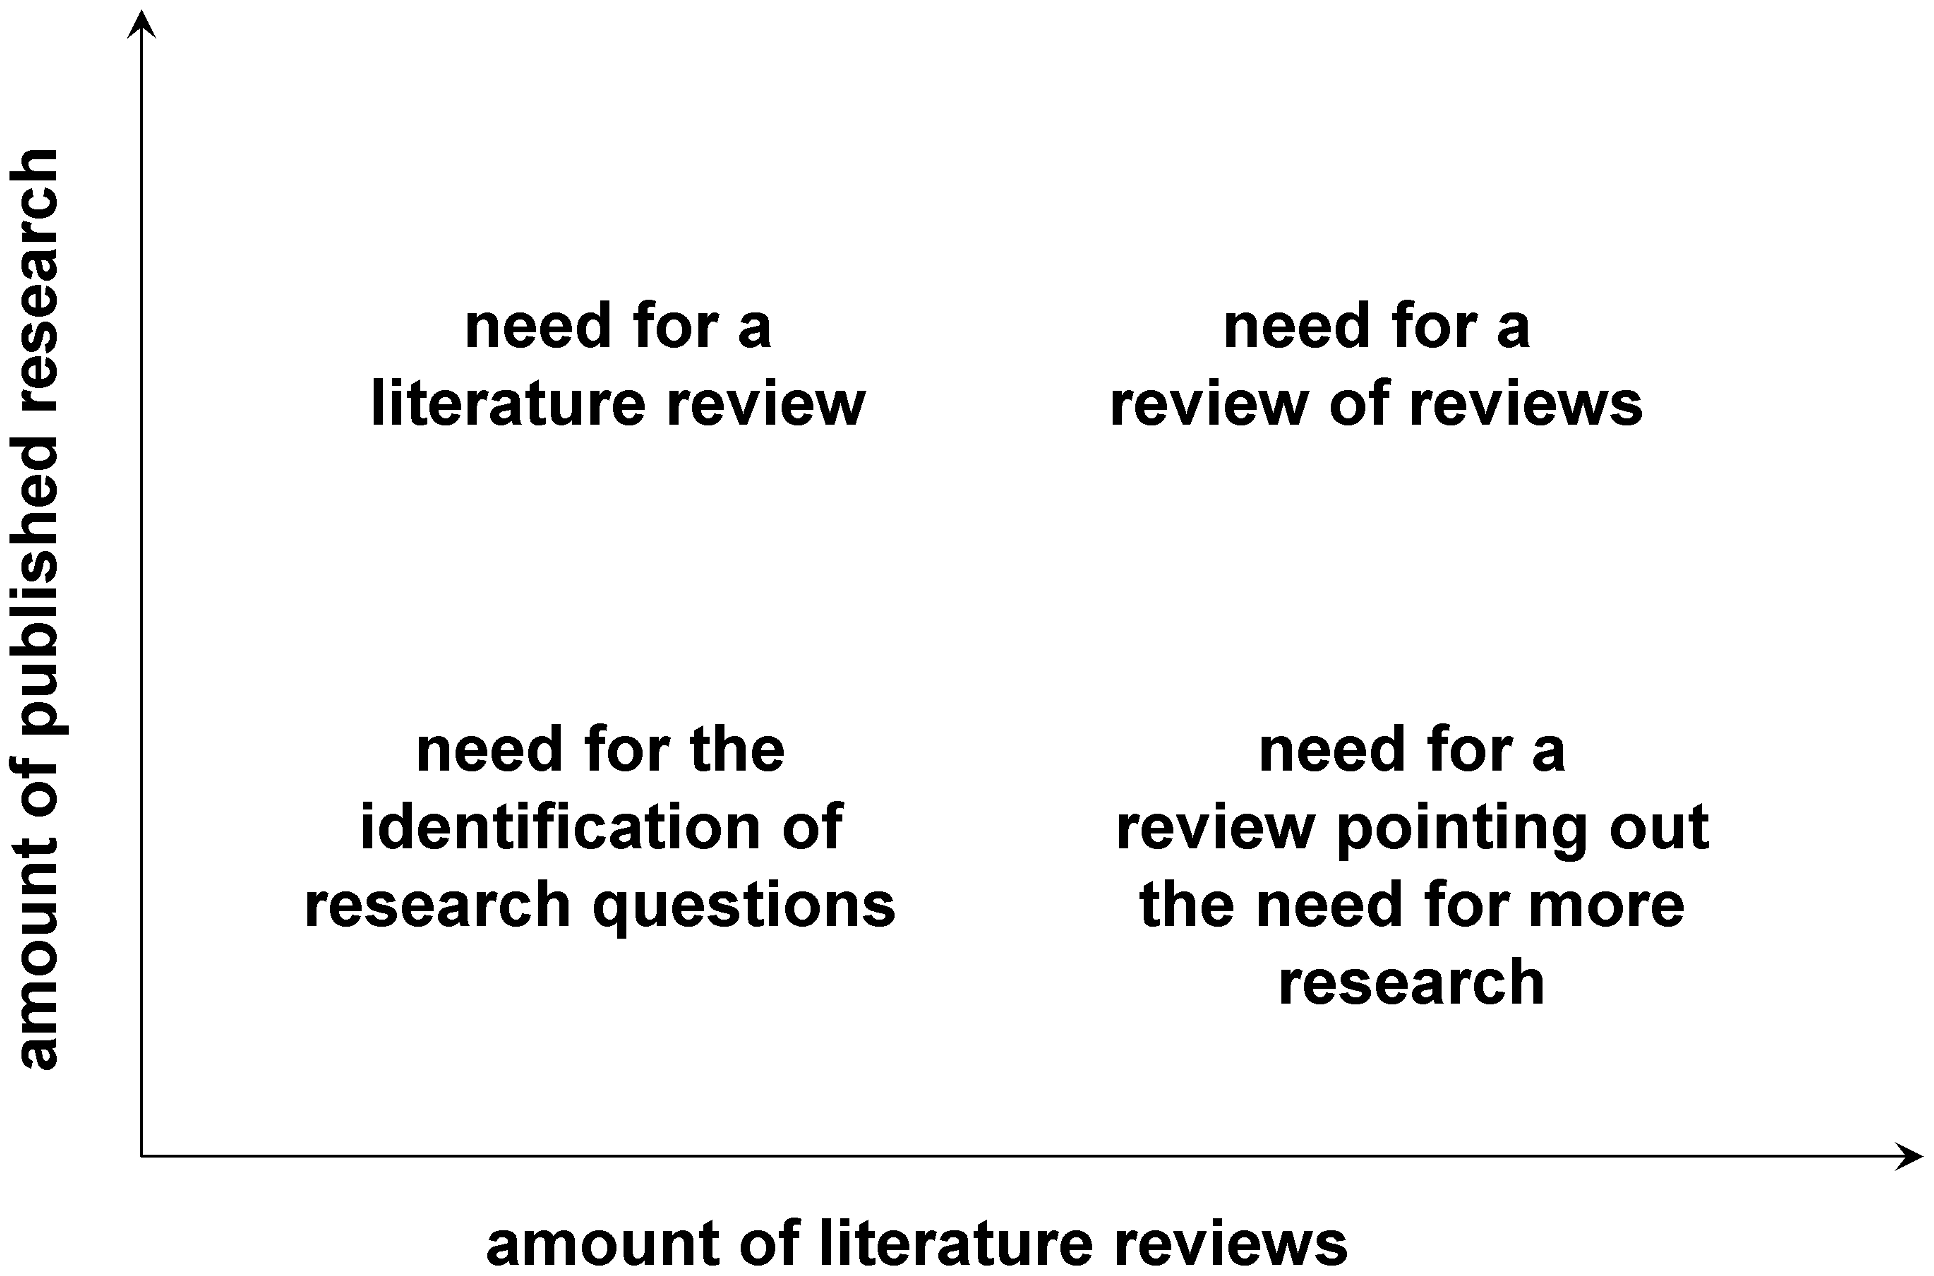
\includegraphics[height=0.8\textheight]{Revisao_resumo/10_dicas_revisao}
\end{frame}

\begin{frame}{10 dicas para um artigo de revisão}
  \begin{enumerate}
  \item Definir tópico e público alvo
  \item Pesquisa abrangente na literatura
  \item Faça anotações enquanto lê
  \item Escolha o tipo de revisão
  \item Texto focado mas de interesse abrangente
  \item Seja crítico e consistente
  \item Estrutura lógica
  \item Peça feedback
  \item Inclua suas publicações, mas seja objetivo
  \item Seja atual, mas não esqueça os estudos ``clássicos''
  \end{enumerate}
Fonte: PLOS
\end{frame}

\subsection{Aprofundamento}

\begin{frame}{Aprofundamento}
    \begin{block}{Leitura}
    Seções do livro texto: {\bf 4.7}
  \end{block}
\end{frame}

\begin{frame}{Referências}
  \begin{itemize}
  \item<1->
    \url{http://writing.colostate.edu/guides/guide.cfm?guideid=79}
  \item<1-> Ten Simple Rules for Writing a Literature Review
    (Pautasso, 2013) PLOS Comp Biol
%  \item<1-> \url{}
  \end{itemize}
\end{frame}


\section{Resumo}

\subsection{Resumo}

\begin{frame}{Definição}
  \begin{itemize}
  \item Mostra os aspectos principais do trabalho ou projeto
  \item linguagem técnica, sucinto
  \item curto
  \end{itemize}
\end{frame}

\subsection{Objetivos}

\begin{frame}{Objetivos do resumo}
  \begin{itemize}
  \item Ajudar o leitor a decidir se ele deve ler o texto completo

%O leitor vai usar o abstract de artigos quando for fazer o levantamente bibliográfico.

  \item Ajudar o leitor a lembrar fatos importantes de um assunto

%Depois de ler vários artigos, pode ser difícil para o leitor se lembrar onde uma certa informação ou fato foi obtido, para fins de citação

  \item Ajudar o leitor a entender um texto difícil (pré-leitura
    sumária)

  \item Indexar artigos para fácil localização e referência

  \item Permitir que supervisores se mantenham atualizados na produção
    do lab
  \end{itemize}
\end{frame}

\subsection{Tipos}

\begin{frame}{Tipos de resumo}
  \begin{itemize}
  \item Resumo descritivo
  \item Resumo estruturado (informativo)
  \end{itemize}
\end{frame}

\begin{frame}{Resumo descritivo}
  \begin{itemize}
  \item Descreve os principais tópicos do texto
  \item ``sumário em forma de parágrafo''
  \item não substitui a leitura do texto
  \end{itemize}
\end{frame}

\begin{frame}{Resumo descritivo}
  \begin{example}
    We continue to document all major climatic variables in the
    uplands and floodplains at Bonanza Creek. In addition, we have
    documented the successional changes in microclimate in 9
    successional upland and floodplain stands at Bonanza Creek (BNZ)
    and in four elevational locations at Caribou-Poker Creek
    (CPCRW). A sun photometer is operated cooperatively with NASA to
    estimate high-latitude atmospheric extinction coefficients for
    remote-sensing images. Electronic data are collected monthly and
    loaded into a database which produces monthly summaries.  (...)
  \end{example}
  ``Bonanza Creek LTER [Long Term Ecological Research] 1997 Annual
  Progress Report''

\end{frame}

\subsection{Resumo informativo}

\begin{frame}{Resumo informativo}
  \begin{itemize}
  \item Inclui os detalhes essenciais do texto
  \item É suficiente para a decisão de ler ou não o texto completo
  \item Pode ser usado para mapear informações, fatos e dados
  \item Mais usado para artigos experimentais
  \end{itemize}
\end{frame}

\begin{frame}{Resumo informativo}
  Componentes típicos do resumo informativo
  \begin{itemize}
  \item Contexto e/ou motivação
  \item Objetivo, apresentação do problema
  \item Metodologia (para trabalhos experimentais)
  \item Principais resultados e descobertas
  \item Principais conclusões
  \end{itemize}
\end{frame}

\begin{frame}{Resumo informativo}
  Proposta de padronização (CONSORT)
  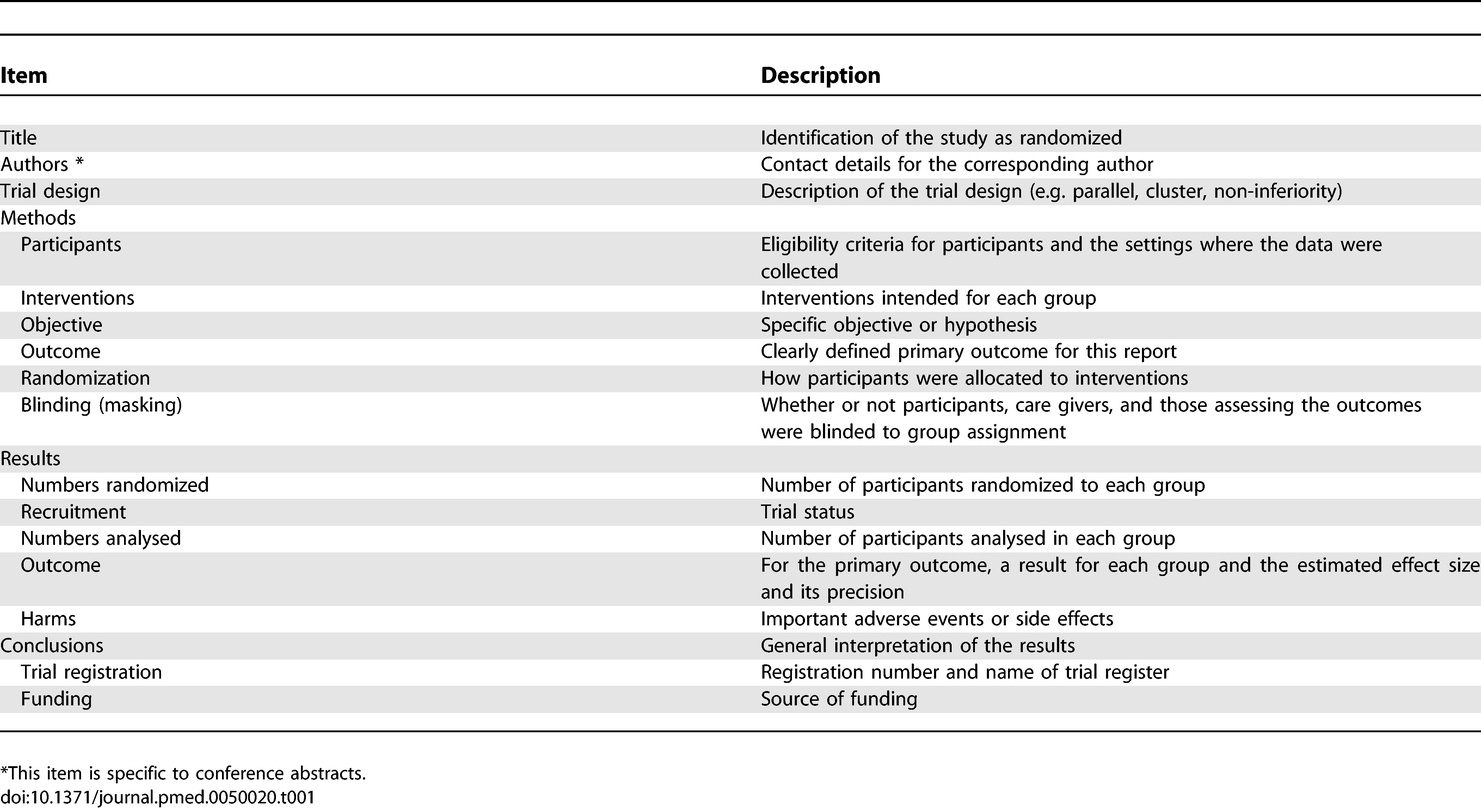
\includegraphics[height=0.8\textheight]{Revisao_resumo/resumo_estruturado}
\end{frame}

\begin{frame}{Resumo informativo}
  \begin{example}
    Research reported by Daly, Miller, and their colleagues suggests
    that writing apprehension is related to a number of factors we do
    not yet fully understand. This study suggests that included among
    those factors should be the belief that writing ability is a
    gift. Giftedness, as it is referred to in the study, is roughly
    equivalent to the Romantic notion of original genius. Results from
    a survey of 247 postsecondary students enrolled in introductory
    writing courses at two institutions indicate that higher levels of
    belief in giftedness are correlated with higher levels of writing
    apprehension, (...) 
  \end{example}
  ``Palmquist, M., \& Young, R. (1992). The Notion of Giftedness and
  Student Expectations About Writing. Written Communication, 9(1),
  137-168.''

\end{frame}

\begin{frame}{Resumo informativo}
  Contexto, motivação
  \begin{example}
    \alert{Research reported by Daly, Miller, and their colleagues
      suggests that writing apprehension is related to a number of
      factors we do not yet fully understand. This study suggests that
      included among those factors should be the belief that writing
      ability is a gift. Giftedness, as it is referred to in the
      study, is roughly equivalent to the Romantic notion of original
      genius.} Results from a survey of 247 postsecondary students
    enrolled in introductory writing courses at two institutions
    indicate that higher levels of belief in giftedness are correlated
    with higher levels of writing apprehension, (...)
  \end{example}
\end{frame}

\begin{frame}{Resumo informativo}
Metodologia
  \begin{example}
    Research reported by Daly, Miller, and their colleagues suggests
    that writing apprehension is related to a number of factors we do
    not yet fully understand. This study suggests that included among
    those factors should be the belief that writing ability is a
    gift. Giftedness, as it is referred to in the study, is roughly
    equivalent to the Romantic notion of original genius. Results from
    \alert{a survey of 247 postsecondary students enrolled in
      introductory writing courses at two institutions} indicate that
    higher levels of belief in giftedness are correlated with higher
    levels of writing apprehension, (...)
  \end{example}
\end{frame}

\begin{frame}{Resumo informativo}
Resultados
  \begin{example}
    Research reported by Daly, Miller, and their colleagues suggests
    that writing apprehension is related to a number of factors we do
    not yet fully understand. This study suggests that included among
    those factors should be the belief that writing ability is a
    gift. Giftedness, as it is referred to in the study, is roughly
    equivalent to the Romantic notion of original
    genius. \alert{Results} from a survey of 247 postsecondary
    students enrolled in introductory writing courses at two
    institutions \alert{indicate that higher levels of belief in
      giftedness are correlated with higher levels of writing
      apprehension,} (...)
  \end{example}
\end{frame}

\subsection{Aprofundamento}

\begin{frame}{Aprofundamento}
    \begin{block}{Leitura}
    Seções do livro texto: {\bf 8.1.9}
  \end{block}
\end{frame}

\begin{frame}{Referências}
  \begin{itemize}
  \item<1-> \url{http://writing.colostate.edu/guides/guide.cfm?guideid=59}
  \item<1->
    \url{http://www.consort-statement.org/extensions?ContentWidgetId=562}
  \item<1-> \url{http://metodologia.org/}
  \end{itemize}
\end{frame}

\end{document}
